\documentclass[slidestop]{beamer}

\usepackage[english]{babel}

\title{Dutch Variant Database: design and implementation}
\providecommand{\myConference}{Lab-J work discussion}
\providecommand{\myDate}{Wednesday, 20 June 2012}
\author{Martijn Vermaat}
\providecommand{\myGroup}{}
\providecommand{\myDepartment}{Department of Human Genetics}
\providecommand{\myCenter}{Center for Human and Clinical Genetics}
\providecommand{\lastCenterLogo}{
%  \raisebox{-0.1cm}{
%    
\includegraphics[height = 1cm]{lgtc_logo}
%  }
}
\providecommand{\lastRightLogo}{
  
\includegraphics[height = 0.7cm]{nbic_logo}
  %\includegraphics[height = 0.8cm]{nwo_logo_en}
}

\usetheme{lumc}

\begin{document}

% This disables the \pause command, handy in the editing phase.
%\renewcommand{\pause}{}

% Make the title page.
\bodytemplate

\frame{
  \frametitle{Dutch Variant Database}
  \tableofcontents
}

\section{Introduction}

\begin{frame}
  \frametitle{Background}
  NGS produces a large number of genomic variants
  \begin{itemize}
    \item Valuable to medical research
    \item Several groups have their own ad-hoc database
    \item Not easily coupled (technically and politically)
  \end{itemize}
  \vspace{1cm}
  Collaboration needed
\end{frame}

\begin{frame}
 \frametitle{Dutch Variant Database}
 (Or: Diagnostic Variant Database)
\end{frame}

\begin{frame}
  \frametitle{Dutch Variant Database}
  Collaboration to share human genomic variants
  \begin{itemize}
    \item Central human genomic variant database
    \item LUMC, UMCU, UMCN, UMCG
    \item Only accessible to collaborators
    \item Using is sharing
    \item Coordinated by NBIC Bio-Assist
  \end{itemize}
\end{frame}

\section{Data model}

\begin{frame}[fragile]
  \frametitle{Variants}
  Agree on one reference genome (hg19)
  \begin{itemize}
    \item Read from a VCF file
    \item SNPs and small INDELs
    \item Genomic location
    \item Reference sequence
    \item Variant sequence
  \end{itemize}
  \vspace{1cm}
  \pause
  \begin{verbatim}
    chr3  1345445  1345445  A   T
    chr5   244534   244535  TT  AC
    chr5   244538   244538  T   C
    ...
  \end{verbatim}
\end{frame}

\begin{frame}
  \frametitle{Coverage}
  To distinguish true negatives from false negatives
  \begin{itemize}
    \item Read from a BED file
    \item Derived from coverage profile (WIGGLE track)
    \item Regions with sufficient coverage
  \end{itemize}
  \begin{center}
    \only<1,2>{\visible<2>{
\includegraphics[width=0.8\textwidth]{coverage1}}}\only<3>{
\includegraphics[width=0.8\textwidth]{coverage2}}\only<4>{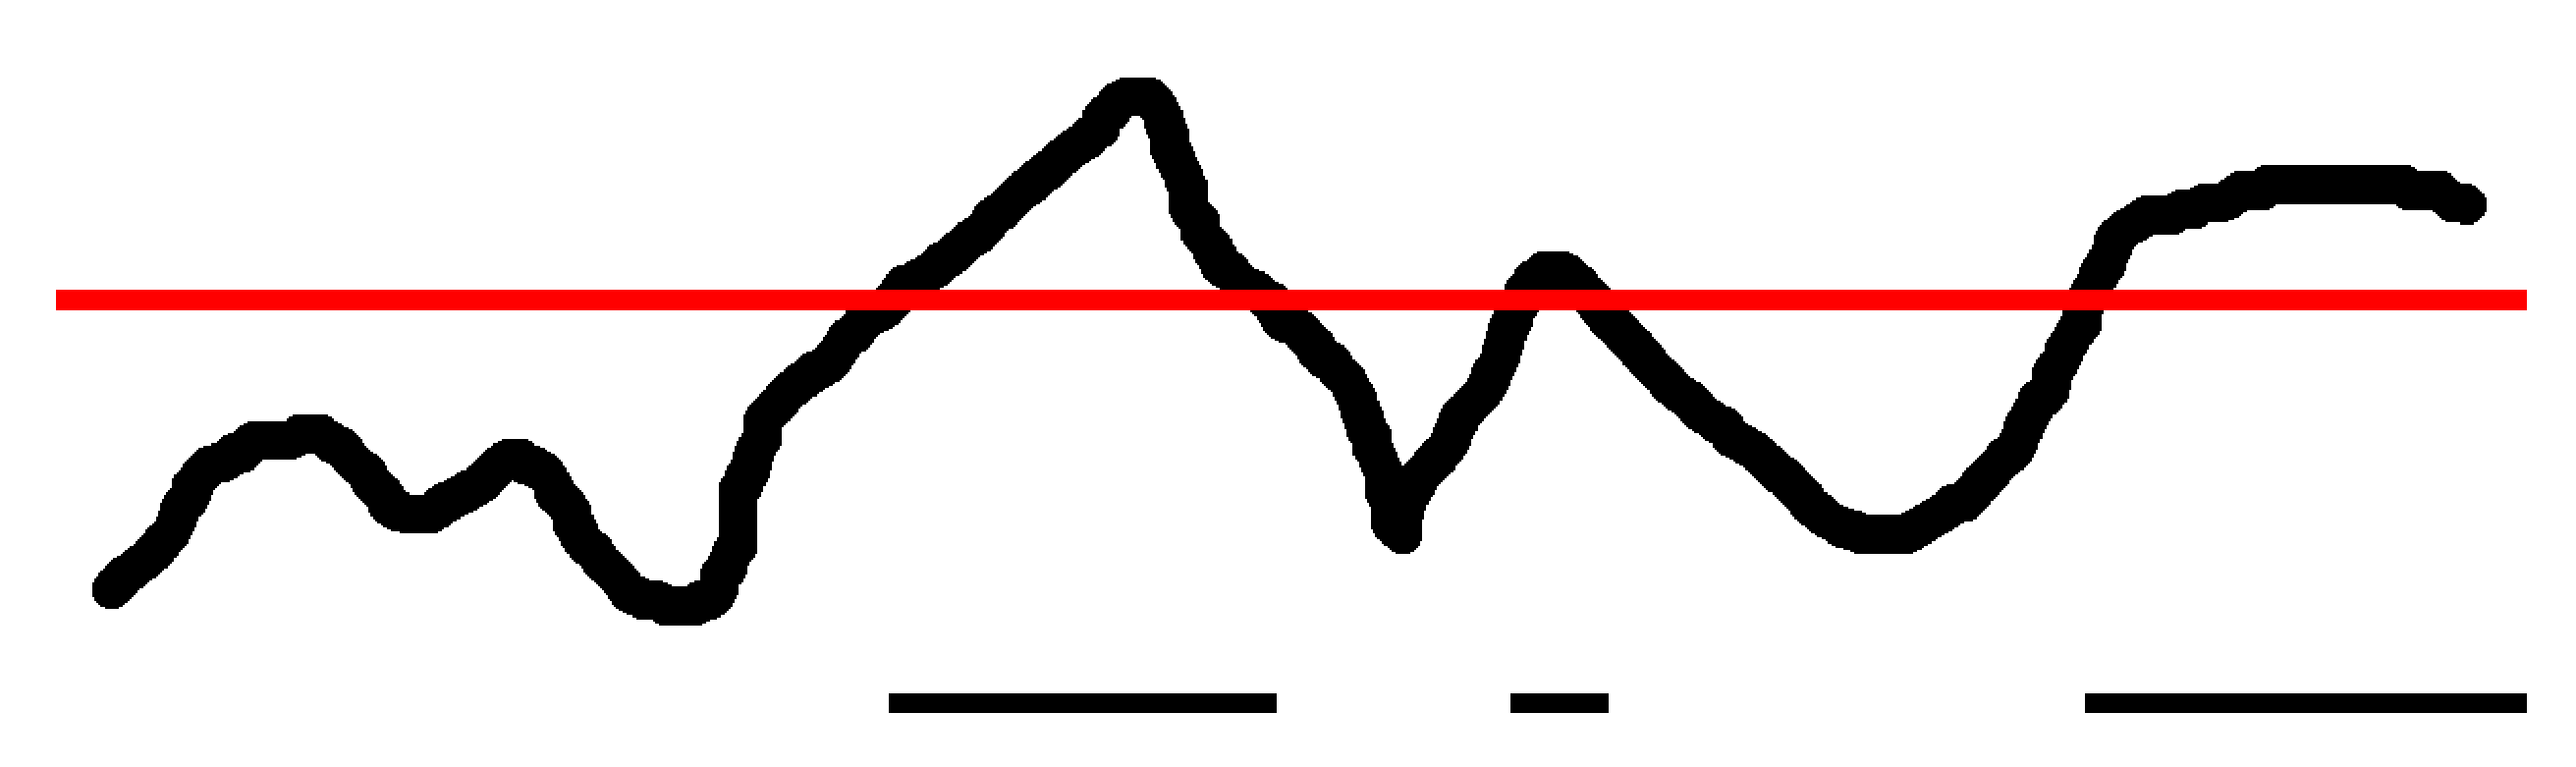
\includegraphics[width=0.8\textwidth]{coverage3}}
  \end{center}
\end{frame}

\begin{frame}
  \frametitle{Coverage example}
  \begin{center}
    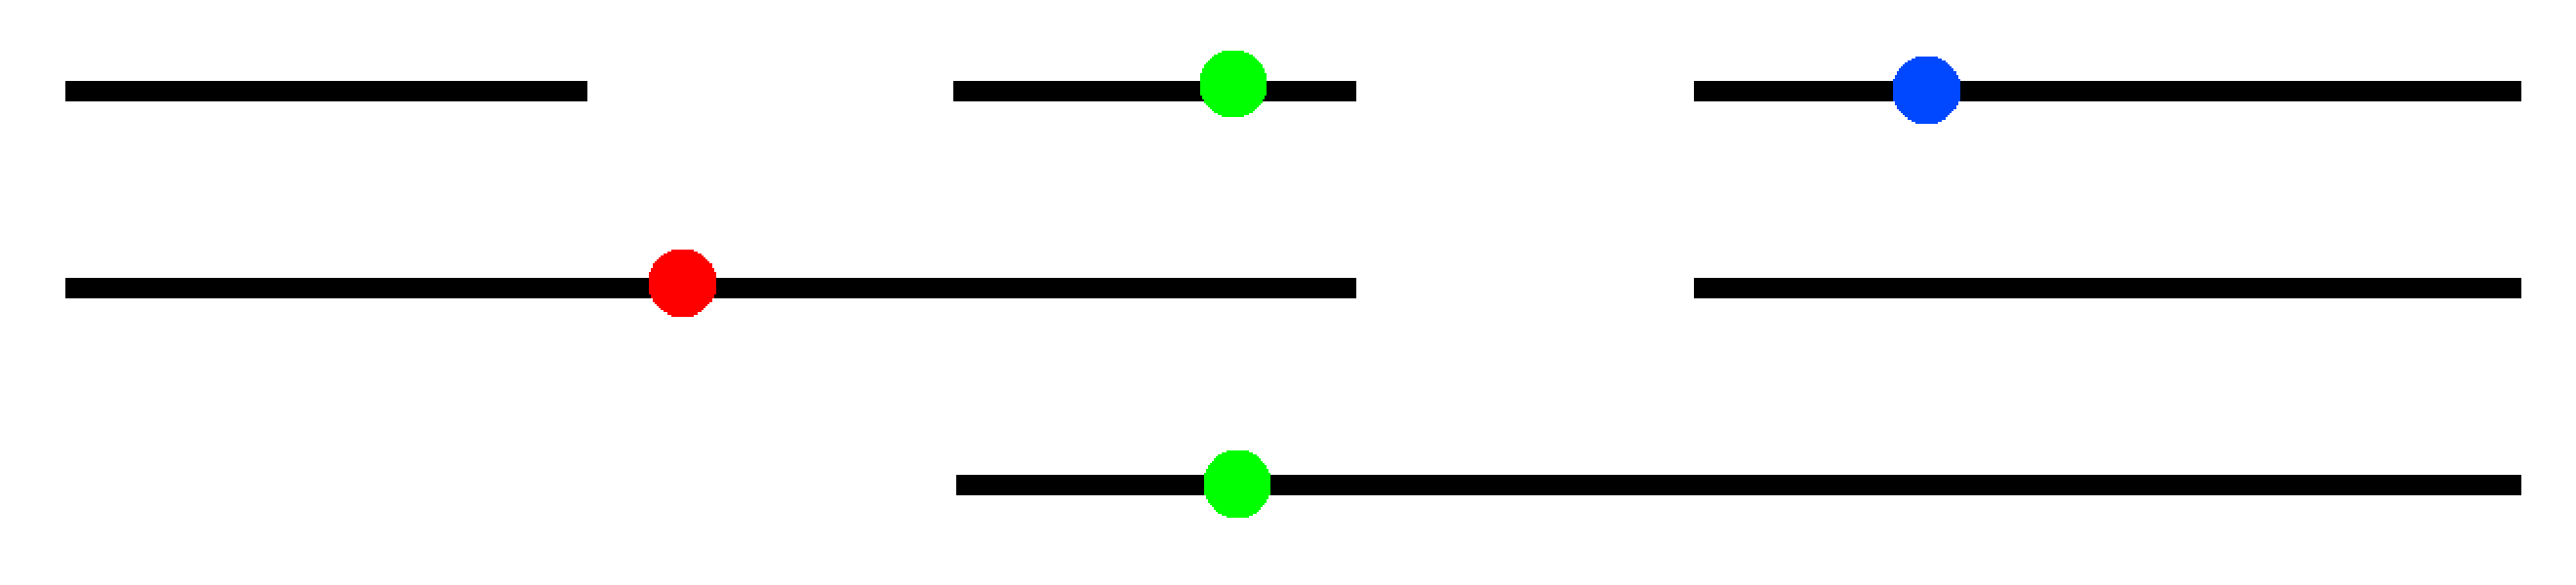
\includegraphics[width=\textwidth]{frequencies}
  \end{center}
\end{frame}

\begin{frame}
  \frametitle{Pooled samples}
  Some samples can only be shared anonymized
  \begin{itemize}
    \item Merge VCF files into one (sorted) VCF file
    \item Keep all coverage tracks
    \item Frequency information can still be calculated
  \end{itemize}
\end{frame}

\begin{frame}
  \begin{center}
    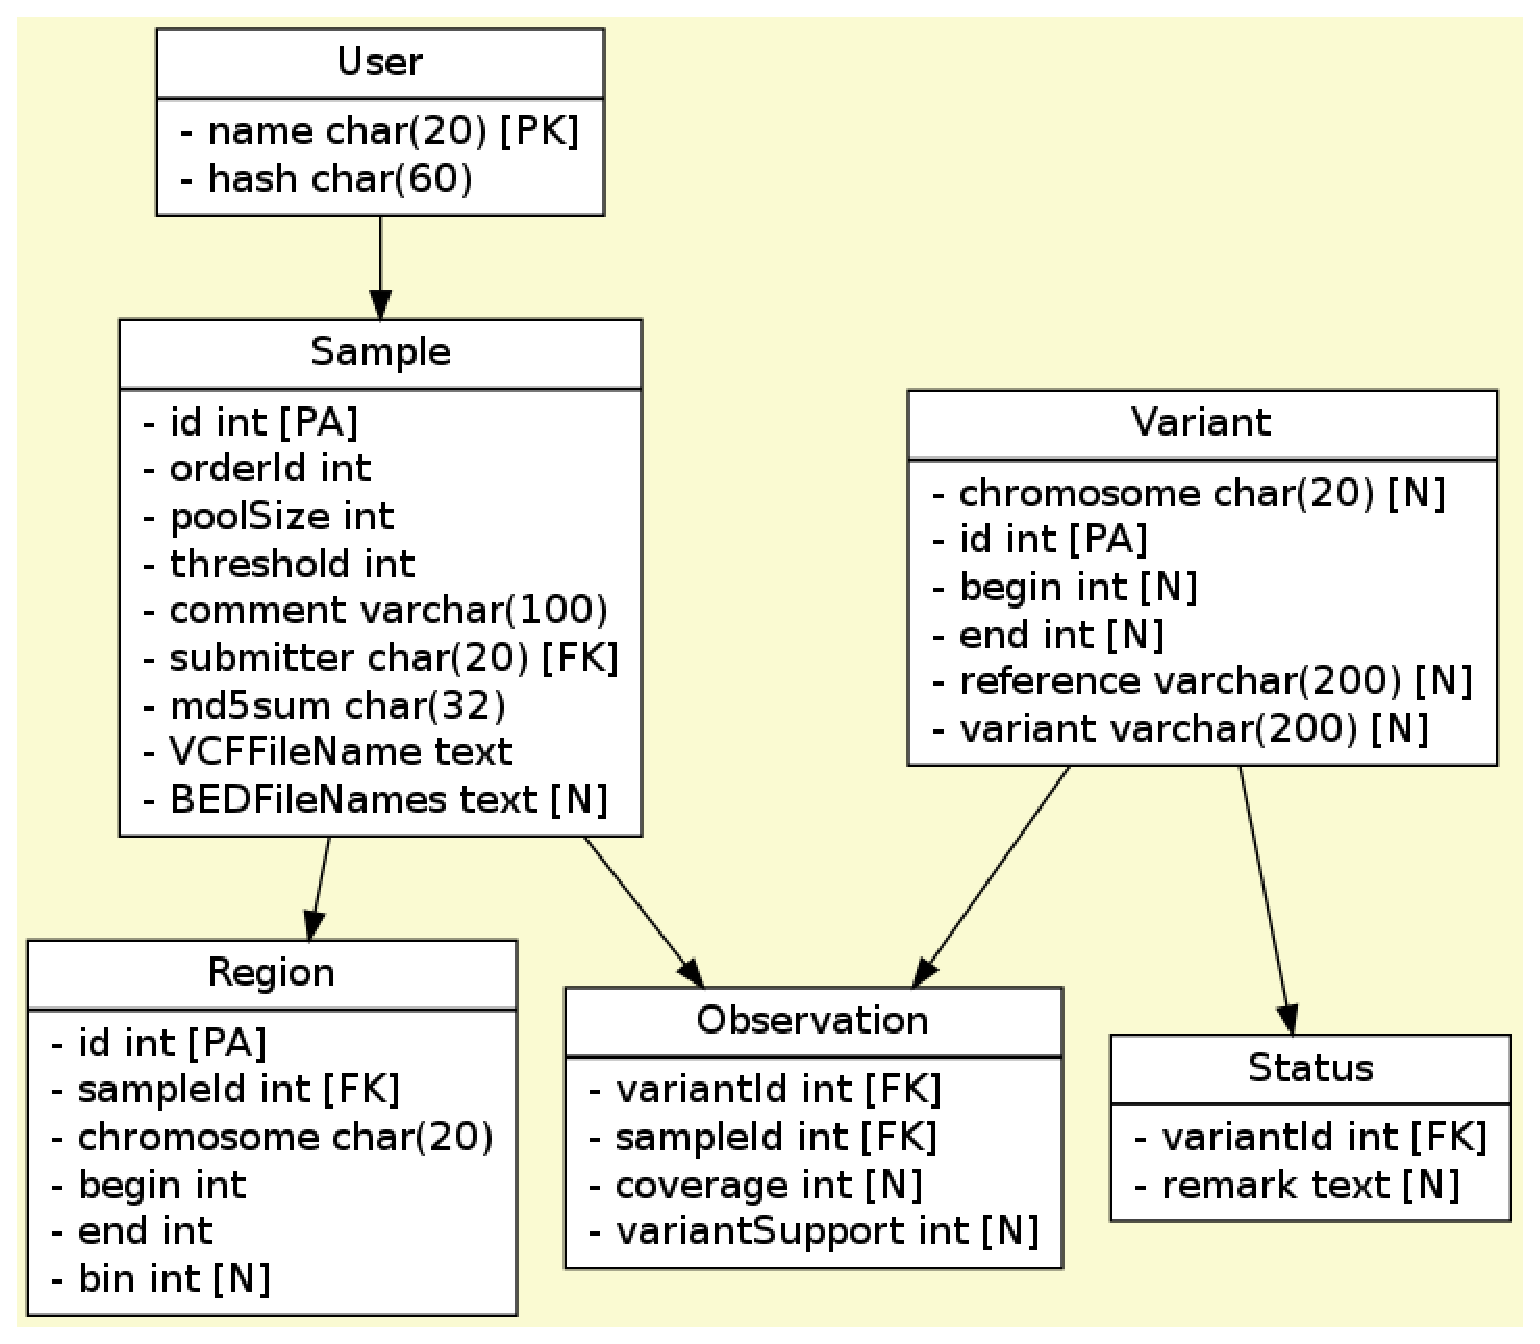
\includegraphics[width=0.8\textwidth]{schema}
  \end{center}
\end{frame}

\section{Using is sharing}

\begin{frame}
  \frametitle{Sample import {\em and} annotation}
  \begin{enumerate}
    \item<1-> Send to the server:
      \begin{itemize}
        \item VCF file with variants
        \item BED file with regions of sufficient coverage
      \end{itemize}
    \item<5-> {\bf Server calculates sample checksum H}
    \item<2-> Server annotates variants with frequencies \uncover<6->{\bf skipping H}
    \item<3-> Download annotation from server
    \item<4-> Server imports variants \uncover<7->{\bf if H is new}
  \end{enumerate}
\end{frame}

\section{Implementation}

\begin{frame}
  \frametitle{Server and client model}
  Central server:
  \begin{enumerate}
    \item MySQL database
    \item SOAP webservice
    \item Implemented in Python
    \item Open Source (AGPL)
  \end{enumerate}
  \vspace{1cm}
  \pause
  User clients:
  \begin{enumerate}
    \item Example implementation available
    \item Conversion from WIG to BED is done locally
    \item Any language speaking SOAP possible
  \end{enumerate}
\end{frame}

\begin{frame}
  \frametitle{Security and privacy}
  Data is sensitive
  \begin{enumerate}
    \item Pooling of samples
    \item Only registered users have access
    \item Server-client communication is encrypted
    \item Only bcrypt hash of passwords stored {\bf*}
  \end{enumerate}
  \vspace{1cm}
  \pause
  {\bf*} bcrypt is designed to be inefficient
\end{frame}

\begin{frame}
  \frametitle{VCF format}
  The VCF file format is more complex than you might think
  \begin{itemize}
    \item Plain text file with tab-separated columns
    \item Chromosome, position, reference, variant columns
    \item INFO and FORMAT columns described in the header
    \item Different ways to encode variant frequency
  \end{itemize}
\end{frame}

\begin{frame}[fragile]
  \frametitle{VCF format example}
  {\tiny
  \begin{verbatim}
##fileformat=VCFv4.0
##fileDate=20090805
##source=myImputationProgramV3.1
##reference=1000GenomesPilot-NCBI36
##phasing=partial
##INFO=<ID=NS,Number=1,Type=Integer,Description=''Number of Samples With Data''>
##INFO=<ID=DP,Number=1,Type=Integer,Description=''Total Depth''>
##INFO=<ID=AF,Number=.,Type=Float,Description=''Allele Frequency''>
##INFO=<ID=AA,Number=1,Type=String,Description=''Ancestral Allele''>
##INFO=<ID=DB,Number=0,Type=Flag,Description=''dbSNP membership, build 129''>
##INFO=<ID=H2,Number=0,Type=Flag,Description=''HapMap2 membership''>
##FILTER=<ID=q10,Description=''Quality below 10''>
##FILTER=<ID=s50,Description=''Less than 50% of samples have data''>
##FORMAT=<ID=GT,Number=1,Type=String,Description=''Genotype''>
##FORMAT=<ID=GQ,Number=1,Type=Integer,Description=''Genotype Quality''>
##FORMAT=<ID=DP,Number=1,Type=Integer,Description=''Read Depth''>
##FORMAT=<ID=HQ,Number=2,Type=Integer,Description=''Haplotype Quality''>
#CHROM POS ID        REF  ALT   QUAL FILTER INFO                  FORMAT NA00001 NA00002 NA00003
20   14370 rs6054257 G    A       29 PASS NS=3;DP=14;AF=0.5;DB;H2 GT:GQ:DP:HQ 0|0:48:1:51,511|0:48:8:51,511/1:43:5:.,.
20   17330 .         T    A       30 q10  NS=3;DP=11;AF=0.017     GT:GQ:DP:HQ 0|0:49:3:58,500|1:3:5:65,30/0:41:3
20 1110696 rs6040355 A    G,T     29 PASS NS=2;DP=10;AF=0.333,0.667;AA=T;DB GT:GQ:DP:HQ 1|2:21:6:23,272|1:2:0:18,22/2:35:4
20 1230237 .         T    .       47 PASS NS=3;DP=13;AA=T         GT:GQ:DP:HQ 0|0:54:7:56,600|0:48:4:51,510/0:61:2
20 1234567 microsat1 GTCT G,GTACT  . PASS NS=3;DP=9;AA=G          GT:GQ:DP    ./.:35:40/2:17:21/1:40:3
  \end{verbatim}}
\end{frame}

\begin{frame}
  \frametitle{PyVCF}
  PyVCF is a Python library for reading VCF files
  \begin{itemize}
    \item Deals with all VCF files
    \item Fast
    \item Being incorporated into BioPython
  \end{itemize}
\end{frame}

\section{Efficient querying}

\begin{frame}
  \frametitle{How indices work}
  Consider a table with 3 columns:
  \begin{itemize}
    \item first name
    \item last name
    \item phone number
  \end{itemize}
  \vspace{0.5cm}
  \pause
  Search on any of the columns, efficiently
  \pause
  \begin{itemize}[<+->]
    \item Solution 1: sort the table
    \item Solution 2: have a separate sorted list of some column(s) with pointers to the table
    \item This is an index
    \item Usually implemented as B-trees
  \end{itemize}
\end{frame}

\begin{frame}
  \frametitle{When indices don't work}
  Consider a table with 2 columns:
  \begin{itemize}
    \item start position
    \item end position
  \end{itemize}
  \vspace{0.5cm}
  \pause
  Search for regions covering some position P, efficiently
  \pause
  \begin{itemize}[<+->]
    \item First find regions with start position smaller than P
    \item In this set, find regions with with end position greater than P
    \item The second part is hard
    \item Simple indices won't help
  \end{itemize}
\end{frame}

\begin{frame}
  \frametitle{Spatial search}
  Searching for regions covering some position is an example of a spatial search
  \begin{itemize}[<+->]
    \item Or: what restaurants are nearby?
    \item Solution: UCSC binning scheme
    \item Essentially the same as R-trees
  \end{itemize}
\end{frame}

\begin{frame}
  \frametitle{Spatial search}
  Alternative solutions?
  \begin{itemize}[<+->]
    \item Assume regions are of limited length
    \item Assume regions are non-overlapping
    \item 2-column table: position, coverage
    \item Split table on chromosome
    \item Spatial database
  \end{itemize}
  \vspace{1cm}
  \pause
  All have their downsides
\end{frame}

\begin{frame}
  \frametitle{UCSC binning scheme: setup}
  Divide genome into bins where for any two, either:
  \begin{enumerate}
    \item one is contained in the other, or
    \item they are non-overlapping
  \end{enumerate}
  \vspace{0.5cm}
  A region gets assigned the smallest bin in which it fits
  \vspace{0.5cm}
  \begin{center}
    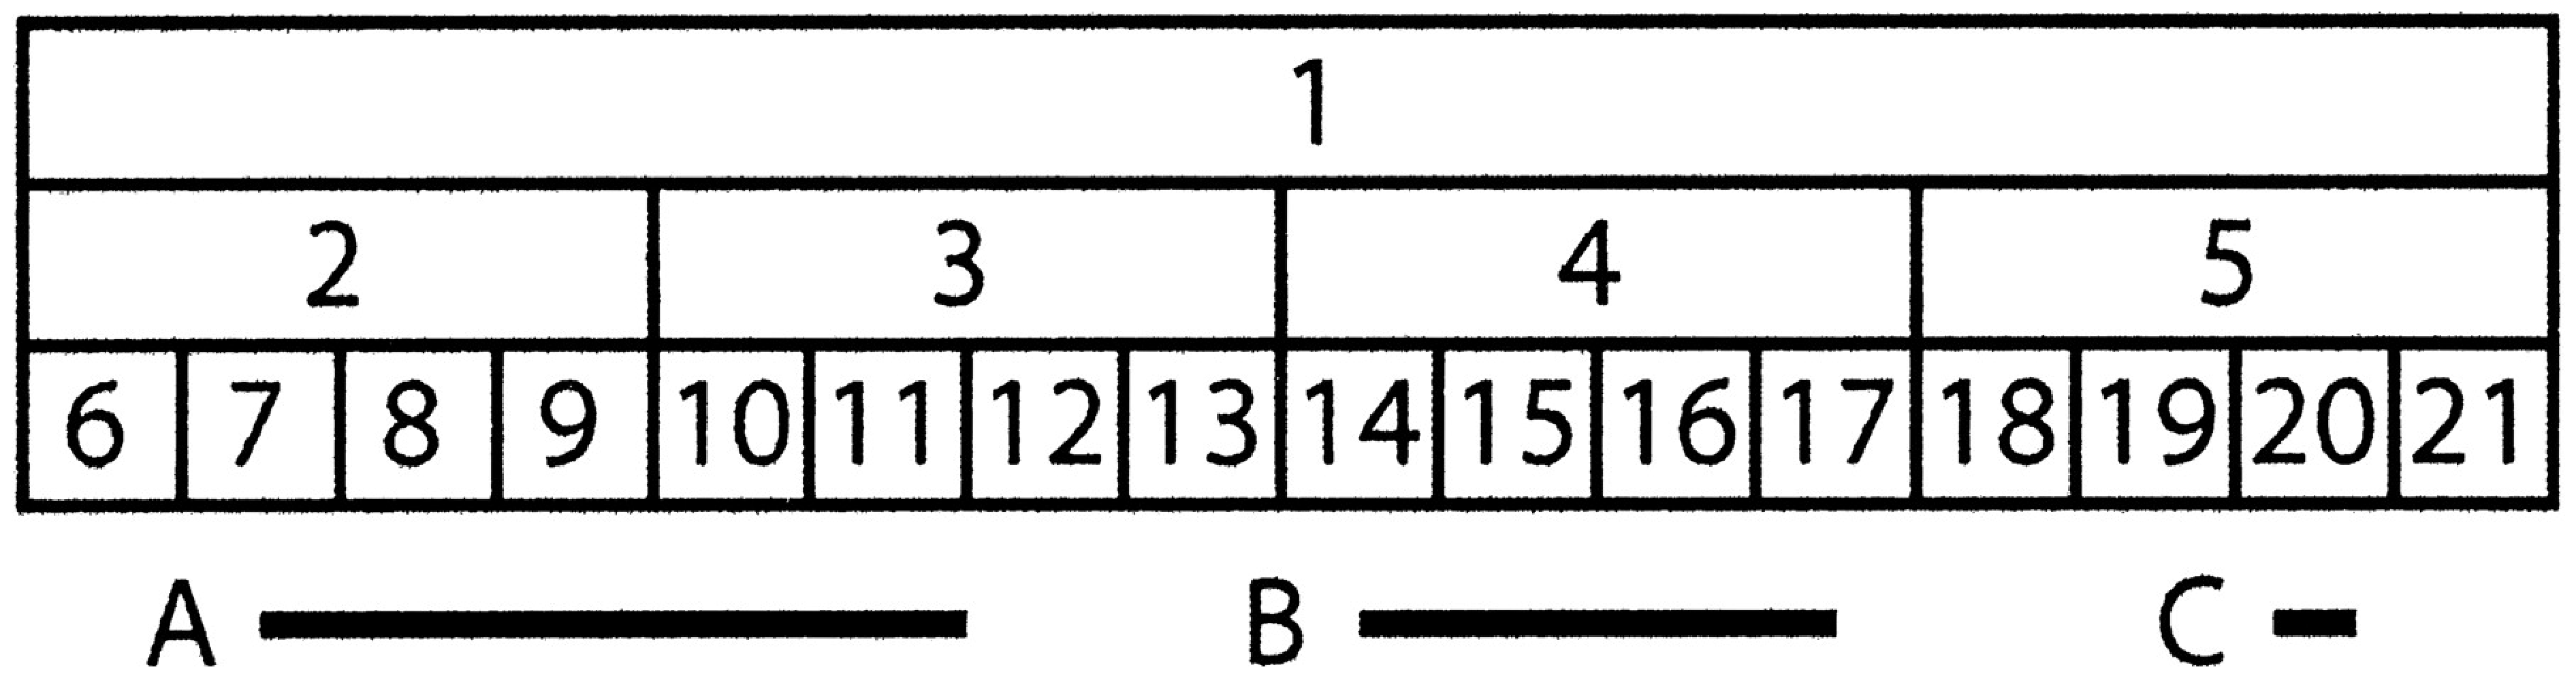
\includegraphics[width=\textwidth]{binning}
  \end{center}
\end{frame}

\begin{frame}
  \frametitle{UCSC binning scheme: spatial search}
  Consider a table with 3 columns:
  \begin{itemize}
    \item start position
    \item end position
    \item bin
  \end{itemize}
  \vspace{0.5cm}
  \pause
  Search for regions covering some position P, efficiently
  \pause
  \begin{itemize}[<+->]
    \item Calculate bins overlapping P
    \item Find regions in these bins
    \item In this set, filter on start and end positions
  \end{itemize}
\end{frame}

\section{Questions?}
\lastpagetemplate
\begin{frame}
  \begin{center}
    Acknowledgements:\\
    \vspace{0.8cm}
    Jeroen Laros\\
    Bradley ten Broeke\\
    Michiel van Galen\\
    \vspace{0.8cm}
    Leon Mei (NBIC)\\
    The rest of the DVD team
  \end{center}
  \vspace{1cm}
  {\tiny
    \begin{enumerate}
      \item Kent et al. The Human Genome Browser at UCSC. Genome Research 2002.12:996-1006
      \item PyVCF: \texttt{github.com/jamescasbon/PyVCF}
      \item DVD: \texttt{trac.nbic.nl/dvd}
    \end{enumerate}
  }
\end{frame}

\end{document}
